% This is samplepaper.tex, a sample chapter demonstrating the
% LLNCS macro package for Springer Computer Science proceedings;
% Version 2.20 of 2017/10/04
%
\documentclass[runningheads]{llncs}
%
\usepackage{graphicx}
% Used for displaying a sample figure. If possible, figure files should
% be included in EPS format.
%
% If you use the hyperref package, please uncomment the following line
% to display URLs in blue roman font according to Springer's eBook style:
% \renewcommand\UrlFont{\color{blue}\rmfamily}

\begin{document}
%
\title{Sensor virtualization for anomaly detection of turbo-machinery sensors - An industrial application} %\thanks{Supported by Baker Hughes.}}
%
%\titlerunning{Abbreviated paper title}
% If the paper title is too long for the running head, you can set
% an abbreviated paper title here
%
%\author{Sachin Shetty\inst{1}\orcidID{0000-0002-0592-8217} %\and
%Valentina Gori\inst{2,3}\orcidID{0000-0003-0215-4022} \and
%Giacomo Veneri\inst{3}\orcidID{0000-0001-9118-8982}}
%
%\authorrunning{F. Author et al.}
% First names are abbreviated in the running head.
% If there are more than two authors, 'et al.' is used.
%
%\institute{
%Baker Hughes, 
%\email{sachin.shetty@bakerhughes.com}
%\and
%Nuovo Pignone Tecnologie (part of Baker Hughes), via Matteucci 2 xxxxx, Firenze, Italy, 
%\email{\{Valentina.Gori, Giacomo.Veneri\}@bakerhughes.com}}
%
\maketitle              % typeset the header of the contribution
%
\begin{abstract}
We apply a Granger causality and auto-correlation analysis to train a Recurrent Neural Network (RNN) that acts as a Virtual sensor model. These models can be used to check the status of several hundreds of sensors during turbo-machinery units’ operation. Checking the health of each sensor is a time-consuming activity. Training a supervised algorithm is not feasible because we don't know all the failure modes that the sensors can undergo. We use a semi-supervised approach and train an RNN (LSTM) on non-anomalous data to build a virtual sensor using other sensors as regressors. We use the Granger causality test to identify the set of input sensors for a given target sensor. We use Auto-correlation Function (ACF) and Partial Auto-correlation Function (PACF) to understand the temporal dependency in data. We then compare the predicted signal vs the real one to raise (in case) an anomaly in real time.

\keywords{Virtual sensor  \and Anomaly detection \and Timeseries multi-regression.}
\end{abstract}
%
%
%
\section{Introduction}
Turbo-machinery units are equipped with hundreds of sensors to monitor their health while functioning \cite{gori2022}. Some of these sensors measure important physical quantities which can affect the overall health of the machine. Thus detecting improper behaviour of sensors or mechanical equipment is a critical task in energy \cite{michelassi2018} and the mechanical industry or, in general, every IOT-related industry \cite{iiot2018}. Detecting unexpected behaviour is also a challenging issue \cite{Hodge2004,gori2022}; indeed, in many real-world problems, samples from the unexpected classes are of insufficient sizes to be effectively modelled using supervised algorithms \cite{Zimek2012}. The task of anomaly detection identifies novelty cases, by training only on samples considered to be normal and then placing these unusual cases \cite{akcay2018ganomaly} \cite{akcay2019skipganomaly} \cite{nanduri2016}. 

\subsection{Problem statement}
In the industry-specific domain,  monitoring some sensors is important and when it triggers an alert it requires machine shutdown and manual inspections, with an associated cost. Sometimes the triggers are false or can be caused by the failure of the sensor rather than a problem with the machine.

We want to detect the fault (anomaly) in the sensor installed on our turbo-machines to prevent unnecessary inspection efforts by site engineering while making sure that correct triggers by sensors are not ignored. Early detection is a required to avoid undesired shutdown.

% (Figure \ref{fig:turbo})
% Please note that the first paragraph of a section or subsection is
% not indented. The first paragraph that follows a table, figure,
% equation etc. does not need an indent, either.

% Subsequent paragraphs, however, are indented.

% \subsubsection{Sample Heading (Third Level)} Only two levels of
% headings should be numbered. Lower level headings remain unnumbered;
% they are formatted as run-in headings.



\section{The Dataset}
% \subsection{A Subsection Sample}
Our data is output from all sensors installed on the turbo-machine and are acquired at a frequency of one sample per second. This includes different kinds of sensors like temperature sensors, pressure sensors, speed sensors etc. Out of these, those sensors which are most important in monitoring the machine status are considered "output sensor" i.e. sensor whose health we want to monitor, to be sure that an eventual alarm triggered by them is actually due to a machine failure, not to a probe failure. The remaining sensors can be used as input sensors for building virtual sensor models (\textit{digital twins}) of the first ones. In this work we will focus on only one target sensor to explain process easily.\\

Our data-set has been collected during 14 months of machine operation (1 second sampling interval).
It has been split into a training set (10 months of data), validation (1 month of data) and test set (3 months), where training data has no reported anomaly (unusual behaviour), while the validation and test sets have some anomalies reported. 

%Subsequent paragraphs, however, are indented.
%\subsubsection{Sample Heading (Third Level)} Only two levels of
%headings should be numbered. Lower level headings remain unnumbered;
%they are formatted as run-in headings.



\section{The Model}
\subsection{Selection of Input Sensor}
There are more than 200 sensors that can be used to build virtual sensors for each output sensor. We used the Granger Causality \cite{granger1969,rosol2022} test to determine the set of input sensors that have a causal effect on each output sensor. With this, we were able to identify around 15 input sensors for given target sensor that can be used to reconstruct the same.

\subsection{Selection of lookback window } 
We use the Auto-correlation to find the temporal relations in both input sensors and target sensor to get the best ``window size'' to train the LSTM model. 
In Fig. \ref{auto-correlation} we can see the Auto-correlation Function (ACF) graph for one of the sensors: there is no significant seasonality but high degree of trend. Hence, we chose sliding window of 5 for this sensor. 

\begin{figure}[t]
\centering
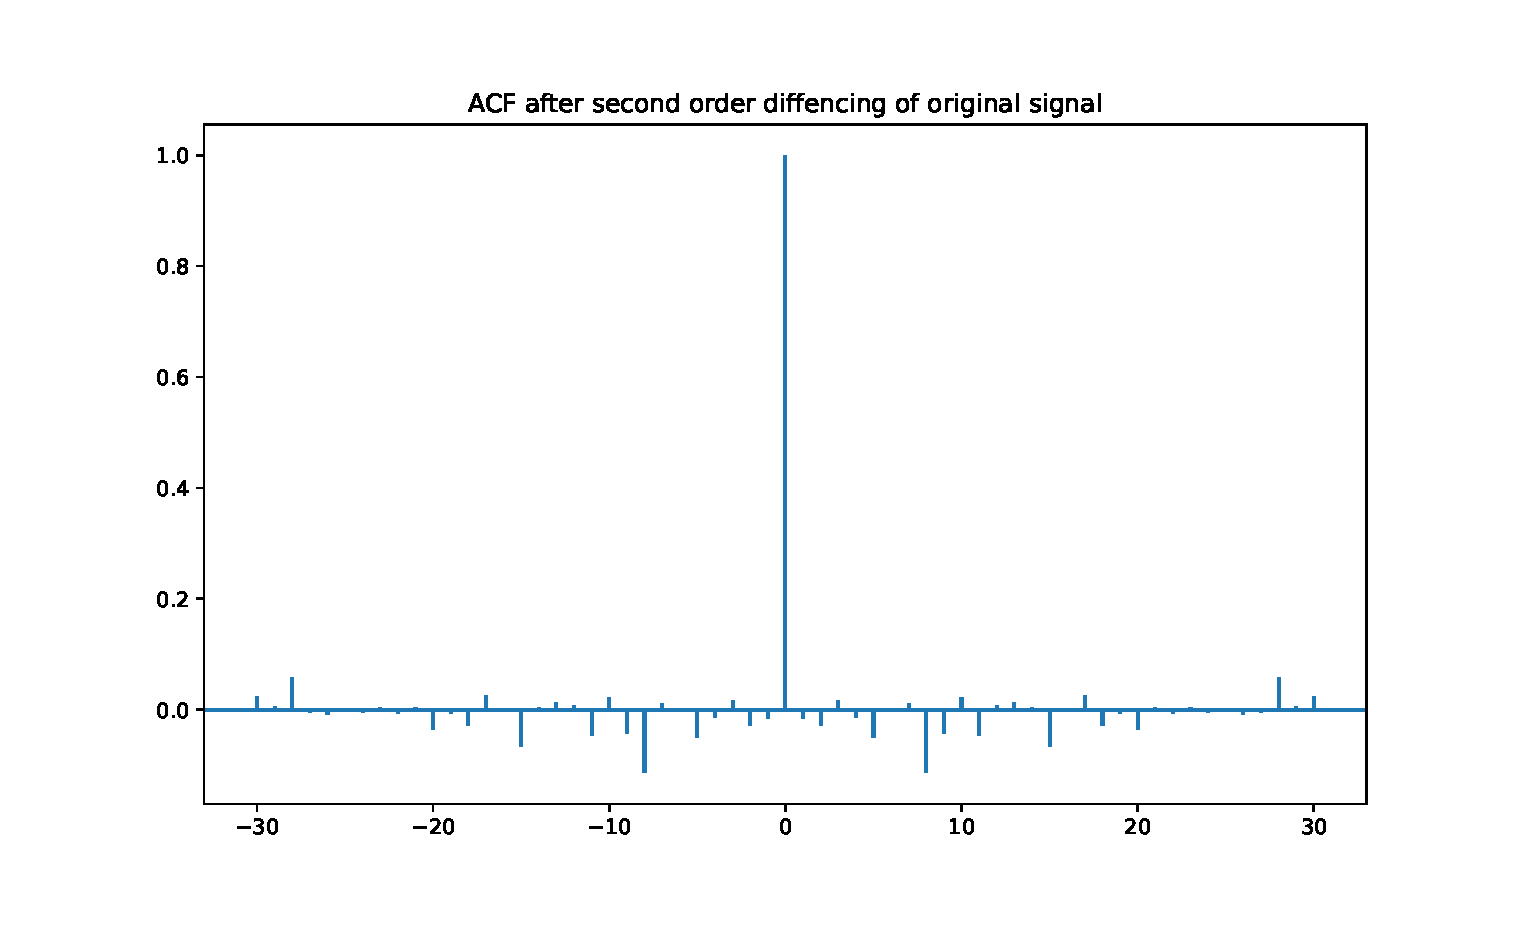
\includegraphics[width=0.7\textwidth]{acf.eps}
\caption{Auto-correlation in one of target sensor.} \label{auto-correlation}
\end{figure}

\newpage

\subsection{Model training} 
We used Deep Learning model with two Long Short-Term Memory (LSTM) layers of 32 nodes each, with \textit{tanh}
activation, followed by 4 Fully Connected layers with \textit{ReLU} activation.
We used Adam optimizer to train the model and a callback on a validation set to 
stop the training.
We used a semi-supervised \cite{gori2022} approach and trained the model on non-anomalous data only, in order to build a virtual sensor acting like a digital twin of the sensor itself \cite{malhotra2015}.
In Fig.~\ref{training} we can see that the model is able to correctly reproduce the actual signal.

\begin{figure}[h]
\centering
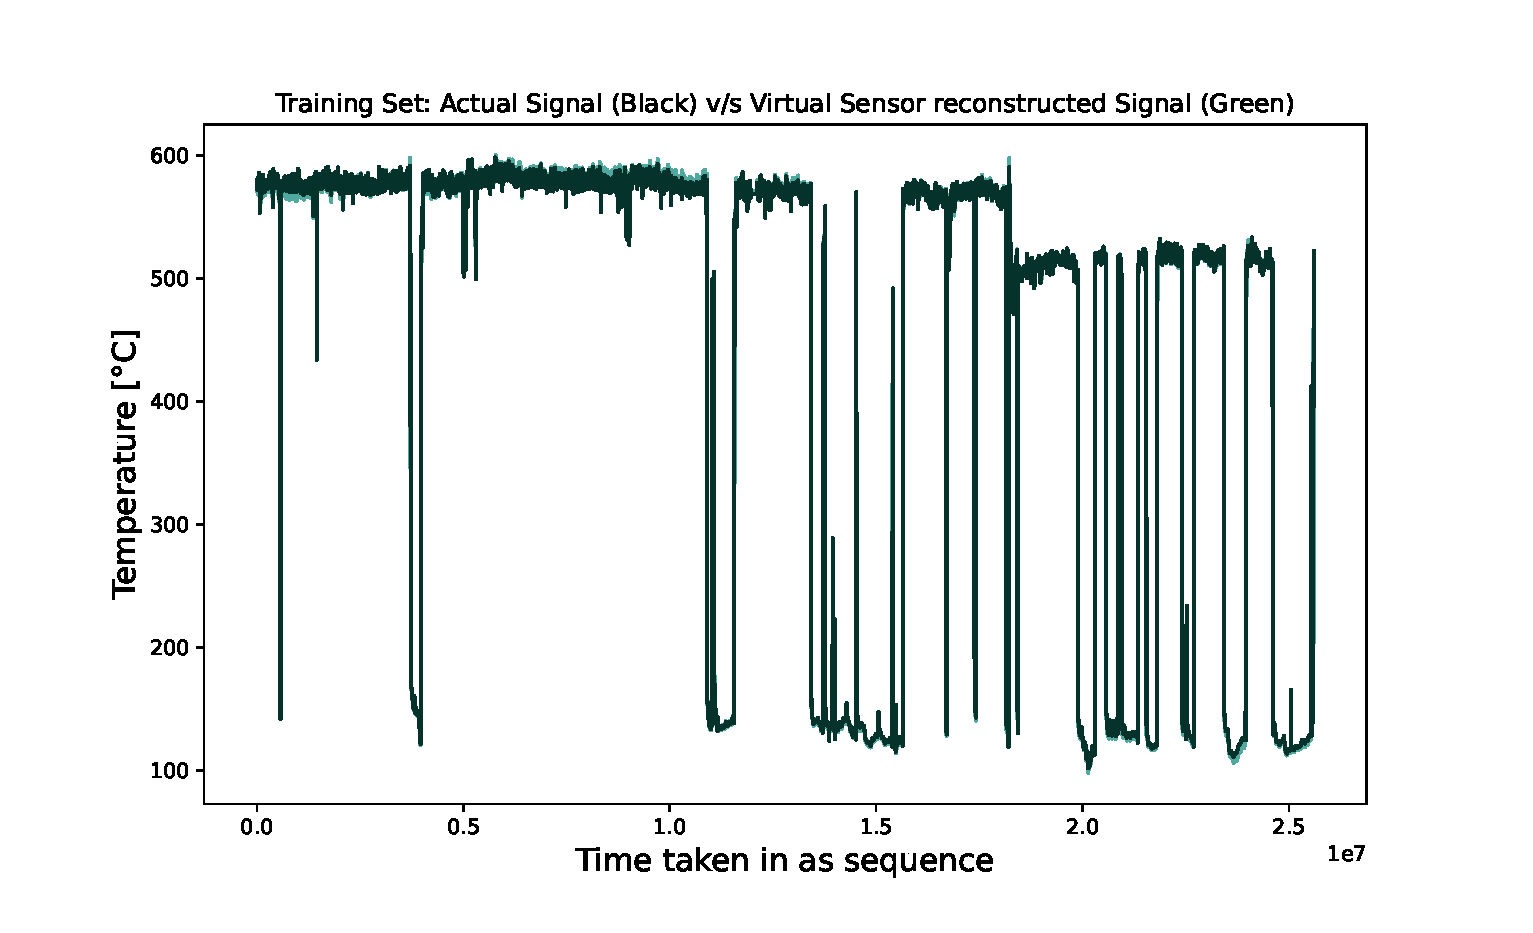
\includegraphics[width=0.75\textwidth]{myfig.eps}
\caption{The picture shows the good fitting between virtual sensor (in orange) and actual sensor (in blue), for the training set. Scale of values has been modified to maintain data confidentiality.}\label{training}
\end{figure}

\newpage

\subsection{Inference Logic} 
Once model is trained, we use it to reconstruct the signal in a time region when sensor anomalies may have occurred.
In order to distinguish anomalous from non-anomalous samples, we need to identify a criterion on virtual vs actual agreement, so that we can declare as anomalous those samples for which the reconstruction error is higher than expected, according to the identified criterion. We decided to use a threshold on the reconstruction error as our criterion. In order to identify this threshold, we used our validation set which has some sample of non-anomalous and some sample of anomalous data point. Fig.~\ref{threshold} shows the distribution of the deviation between actual and reconstructed signal in case of anomalous and non-anomalous points.

\begin{figure}[h]
\centering
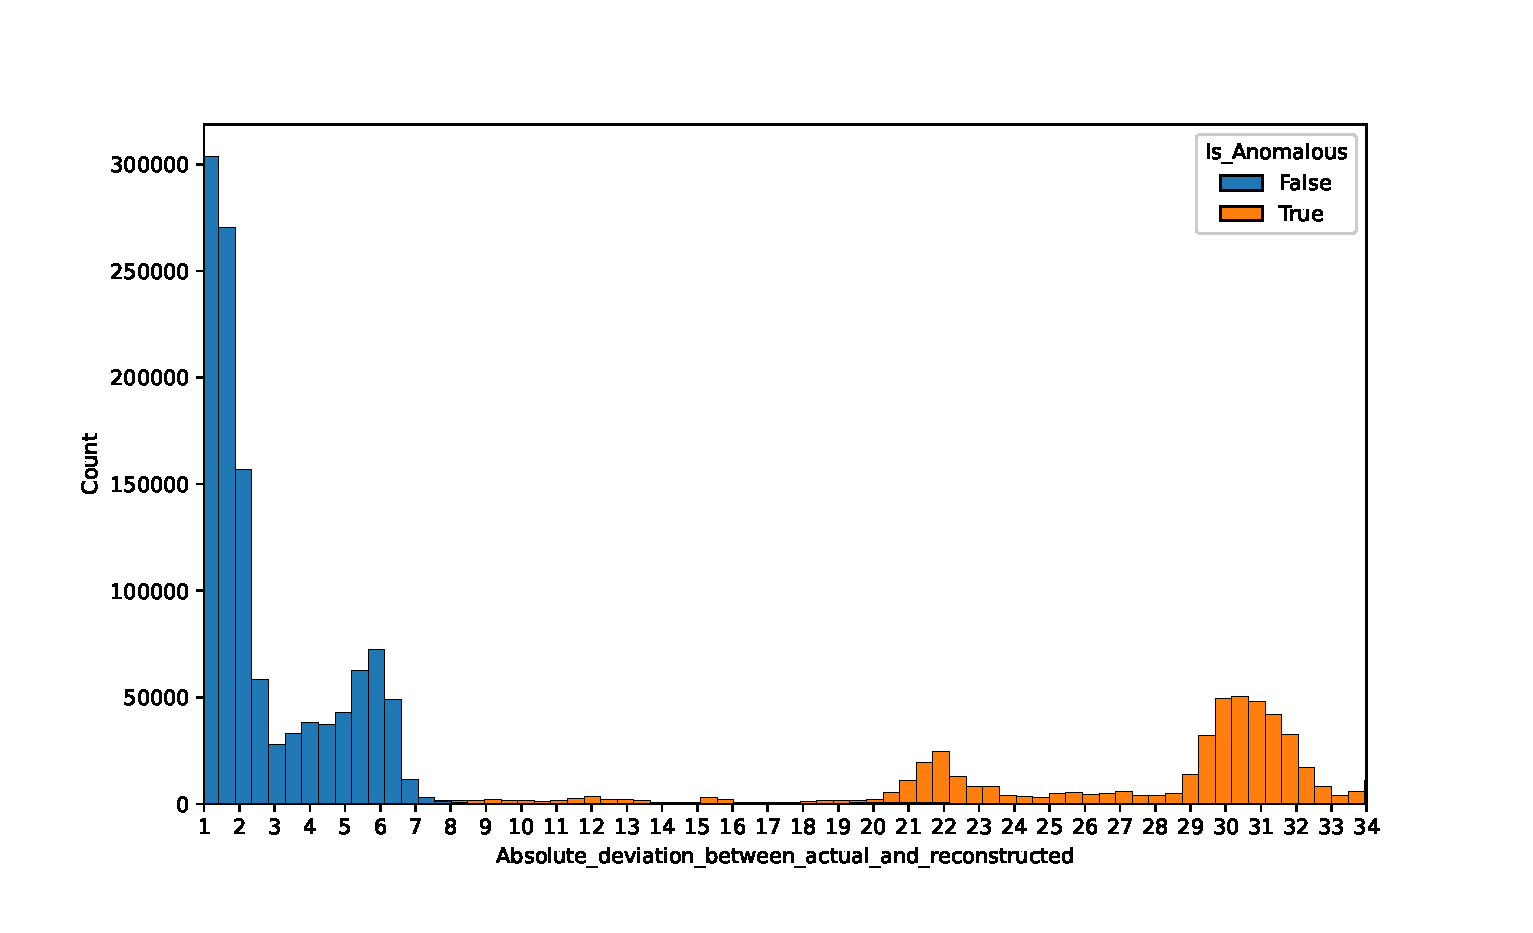
\includegraphics[width=0.65\textwidth]{deviation_plot.eps}
\caption{Deviation between actual and reconstructed signal in validation set.} \label{threshold}
\end{figure}


In this example we can see two non-overlapping distributions: here we decided to use a threshold of $10$. Another possibility is to leverage on the ROC curve to identify the optimal value for the threshold. \\
Figure~\ref{inference} shows that trained model has good reconstruction performance also at test time, when applied to test data where no sensor anomalies occurred (rightmost part of the plot) while, instead, a discrepancy between actual and reconstructed signal is present when model is applied to test data where sensor anomalies are present (leftmost part of the plot).

\begin{figure}[h]
\centering
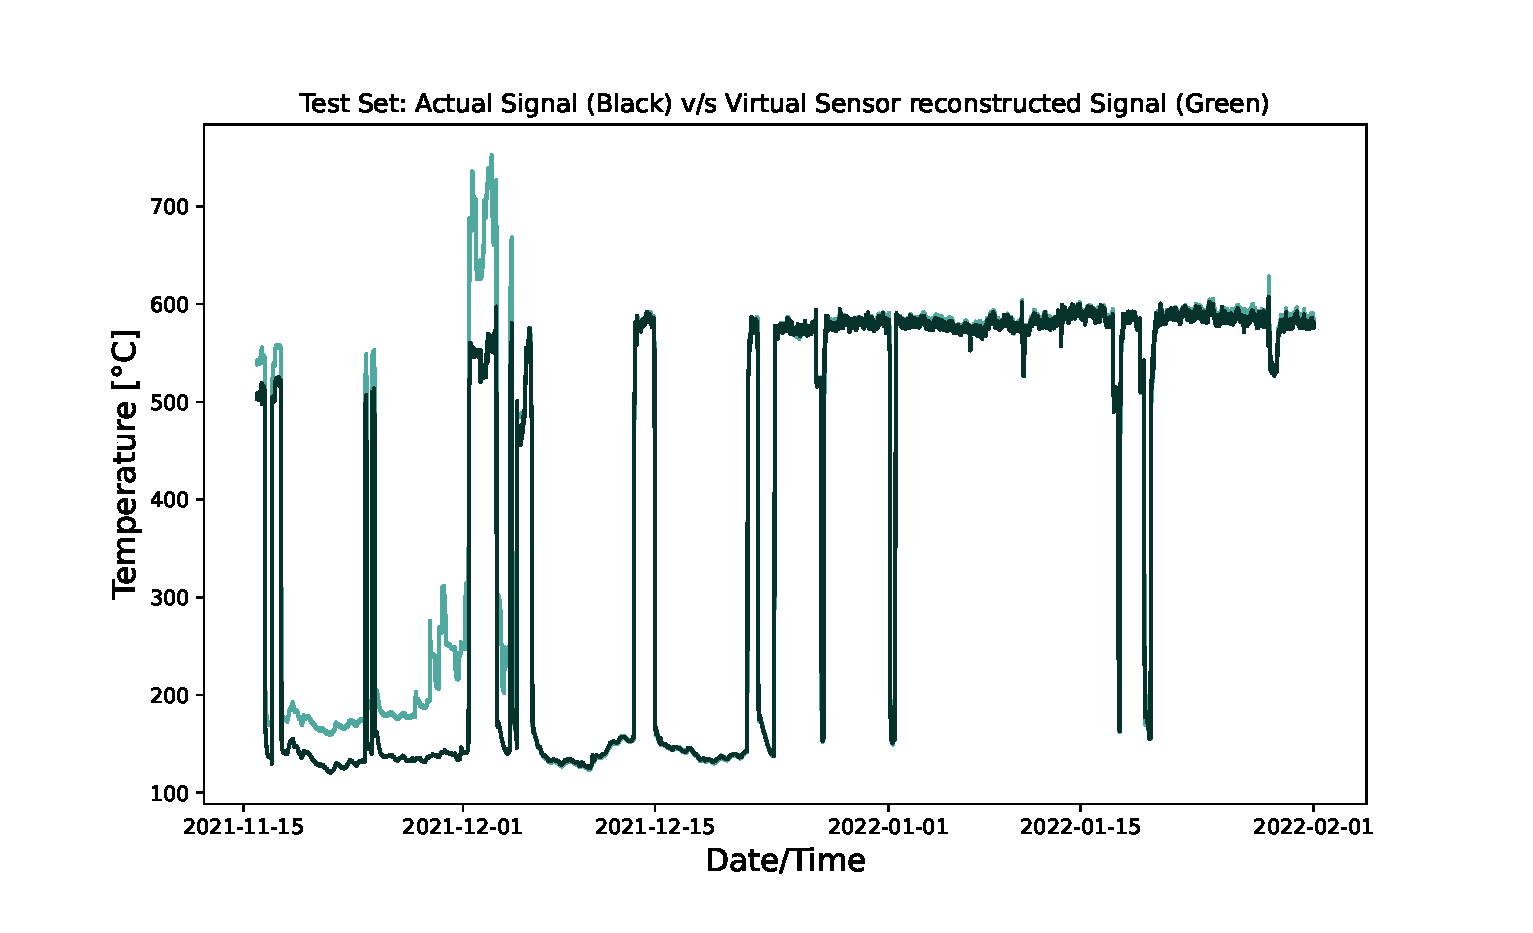
\includegraphics[width=\textwidth]{test_plot.eps}
\caption{The picture shows the superposition of the actual signal (light green) and the reconstructed one (dark green). The region ranging from mid November to early December shows a discrepancy between the two: here a sensor anomaly is highlighted by the model and confirmed by subject matter experts (SME's).
The remaining part of the test set shown here have no anomalies highlighted by the model (very good agreement), nor by SME's. \textit{Scale of values has been modified to maintain data confidentiality}.}\label{inference}
\end{figure}

\newpage
\section{Results}
Tab.~\ref{model_performance} shows reconstruction performance of the model on training, validation and test set (for the latter two, on subsets where no anomalies are occurring). 
Having defined the error $\Delta$ as the deviation between actual signal $y$ and reconstructed signal $\hat{y}$:
\begin{equation}
\Delta = y - \hat{y}
\end{equation}
ME is the mean error, MAPE is the mean absolute percentage error, while
P90 is the 90\textsuperscript{th} percentile of the absolute value of the error.

\begin{table}
\setlength{\tabcolsep}{1em}
\centering
\renewcommand{\arraystretch}{1.2}% for the vertical padding
\caption{Model performance on training, validation and test set.}\label{model_performance}
\begin{tabular}{|l|l|l|l|}
\hline
  & ME & MAPE & P90\\
\hline
Training set & 0.124 & 0.609 & 5.06\\
Validation set (non anomalous samples only) &  1.45 &  1.61  &  5.975 \\
Test set (non anomalous samples only) &  1.89 &  0.647  &  6.52\\ 
\hline
\end{tabular}
\end{table}

For what concerns the anomaly detection performance, when applying the model on test set we where able to detect anomalous signal with precision of 96\% and recall of 100\%, as summarized in Tab.~\ref{ad_performance}.

\begin{table}
\setlength{\tabcolsep}{1em}
\centering
\renewcommand{\arraystretch}{1.2}% for the vertical padding
\caption{Anomaly detection performance summary.}\label{ad_performance}
\begin{tabular}{| c | c | c |}
\hline
      &       Precision      &       Recall      \\
\hline
Full test set & 96\% & 100\%\\
\hline
\end{tabular}
\end{table}


% \begin{figure}[h]
% 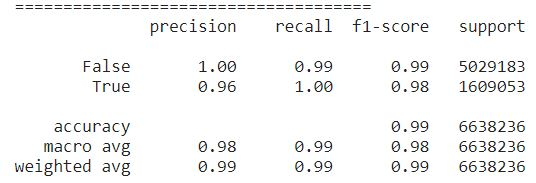
\includegraphics[width=\textwidth]{Accuracy.JPG}
% \caption{Accuracy metric on test set} \label{fig5}
% \end{figure}



% \begin{figure}
% \includegraphics[width=\textwidth]{fig1.eps}
% \caption{A figure caption is always placed below the illustration.
% Please note that short captions are centered, while long ones are
% justified by the macro package automatically.} \label{fig1}
% \end{figure}


% the environments 'definition', 'lemma', 'proposition', 'corollary',
% 'remark', and 'example' are defined in the LLNCS documentclass as well.
%


\section{Conclusions}

In this work we have shown a semi-supervised Deep Learning technique which can be used to perform anomaly detection in an industrial context. In particular, we have applied anomaly detection to turbo-machinery units by training a virtual sensor model for a given sensor. We first selected input features through Granger causality and leveraged auto-correlation and partial auto-correlation functions to identify window size for the recurrent neural network chosen (LSTM).\\
This method can be scaled and extended to almost all the sensors installed on the unit, for a complete sensor anomaly detection system.
Furthermore, once the model has been trained for a single sensor, we can later retrain the model using data collected over time, using a continual learning approach~\cite{rebuffi2017icarl}, so that the algorithm is able to also take into account data shift phenomena.
Our next plans focus on the deployment of the inference algorithm on edge devices (on MarkVIe system). For this purpose, some model distillation  may be required (for a review~\cite{gou2021}). In particular, we need to detect potential fault of sensor earlier, so that we can exclude the sensor from the control and avoiding undesired shutdown.





% For citations of references, we prefer the use of square brackets
% and consecutive numbers. Citations using labels or the author/year
% convention are also acceptable. The following bibliography provides
% a sample reference list with entries for journal
% articles~\cite{ref_article1}, an LNCS chapter~\cite{ref_lncs1}, a
% book~\cite{ref_book1}, proceedings without editors~\cite{ref_proc1},
% and a homepage~\cite{ref_url1}. Multiple citations are grouped
% \cite{ref_article1,ref_lncs1,ref_book1},
% \cite{ref_article1,ref_book1,ref_proc1,ref_url1}.
%
% ---- Bibliography ----
%
% BibTeX users should specify bibliography style 'splncs04'.
% References will then be sorted and formatted in the correct style.
%
% \bibliographystyle{splncs04}
% \bibliography{mybibliography}
%
\begin{thebibliography}{18}

\bibitem{michelassi2018}
    Michelassi, V., Allegorico, C., Cioncolini, S. and Graziano, A. and Tognarelli, L. and Sepe, M.: Machine Learning in Gas Turbines, In: Mechanical Engineering (2018), vol. 140, n. 09, pp S54-S55, 
    https://doi.org/10.1115/1.2018-SEP5, https://asmedigitalcollection.asme.org/memagazineselect/article-pdf/140/09/S54/6352969/me-2018-sep5.pdf

\bibitem{iiot2018}  
Capasso, A.: Hands-On Industrial Internet of Things: Create a Powerful Industrial IoT Infrastructure 
Using Industry 4.0. Packt Publishing (2018)

\bibitem{Hodge2004}
Hodge, V. J., Austin, J.: A Survey of Outlier Detection Methodologies. In: Artificial Intelligence Review,
vol. 22, pp. 85--126, 2004


\bibitem{Zimek2012}
Zimek, A., Schubert, E., Kriegel, H.: A survey on unsupervised outlier detection in high-dimensional numerical data. In: Statistical Analysis and Data Mining: The ASA Data Science Journal, vol. 5, pp 363-387, Wiley Periodicals (2012)


\bibitem{akcay2019skipganomaly}
Akçay, S.,  Atapour-Abarghouei, A., P. Breckon, T.: Skip-GANomaly: Skip Connected and Adversarially Trained Encoder-Decoder Anomaly Detection, 2019


\bibitem{akcay2018ganomaly}
Akçay, S.,  Atapour-Abarghouei, A., P. Breckon, T.: GANomaly: Semi-Supervised Anomaly Detection via Adversarial Training, 2018


\bibitem{nanduri2016}
Nanduri, A., Sherry, L.: Anomaly detection in aircraft data using Recurrent Neural Networks (RNN), 2016 Integrated Communications Navigation and Surveillance (ICNS), 2016, pp 5C2-1-5C2-8

\bibitem{gori2022}
V. Gori, G. Veneri and V. Ballarini, "Continual Learning for anomaly detection on turbomachinery prototypes - A real application," 2022 IEEE Congress on Evolutionary Computation (CEC), Padua, Italy, 2022, pp. 1-7, doi: 10.1109/CEC55065.2022.9870234.

\bibitem{granger1969}
Granger, C. W. J. (1969). Investigating Causal Relations by Econometric Models and Cross-spectral Methods. Econometrica, 37(3), 424–438. https://doi.org/10.2307/1912791

\bibitem{rosol2022}
Maciej Rosoł, Marcel Młyńczak, Gerard Cybulski, Granger causality test with nonlinear neural-network-based methods: Python package and simulation study. Computer Methods and Programs in Biomedicine, Volume 216, 2022, 106669, ISSN 0169-2607, https://doi.org/10.1016/j.cmpb.2022.106669.

\bibitem{malhotra2015}
Malhotra, Pankaj \& Vig, Lovekesh \& Shroff, Gautam \& Agarwal, Puneet. (2015). Long Short Term Memory Networks for Anomaly Detection in Time Series. 

\bibitem{rebuffi2017icarl}
Rebuffi, S.-A., Kolesnikov, A., Sperl G., Lampert, C. H.: iCaRL: Incremental Classifier and Representation Learning. 2017.

\bibitem{gou2021}
Gou, J., Yu, B., Maybank, S.J. et al. Knowledge Distillation: A Survey. Int J Comput Vis 129, 1789–1819 (2021). https://doi.org/10.1007/s11263-021-01453-z

% \bibitem{ref_article1}
% Author, F.: Article title. Journal \textbf{2}(5), 99--110 (2016)

% \bibitem{ref_lncs1}
% Author, F., Author, S.: Title of a proceedings paper. In: Editor,
% F., Editor, S. (eds.) CONFERENCE 2016, LNCS, vol. 9999, pp. 1--13.
% Springer, Heidelberg (2016). \doi{10.10007/1234567890}

% \bibitem{ref_book1}
% Author, F., Author, S., Author, T.: Book title. 2nd edn. Publisher,
% Location (1999)

% \bibitem{ref_proc1}
% Author, A.-B.: Contribution title. In: 9th International Proceedings
% on Proceedings, pp. 1--2. Publisher, Location (2010)

% \bibitem{ref_url1}
% LNCS Homepage, \url{http://www.springer.com/lncs}. Last accessed 4
% Oct 2017


\end{thebibliography}
\end{document}



